\documentclass[11pt,a4paper,landscape]{article}
\usepackage[margin=13mm]{geometry}
\usepackage{fontspec}
\usepackage{xeCJK}
\setmainfont{Arial}
\setCJKmainfont{Yu Gothic}
\usepackage{graphicx,booktabs,xcolor,amsmath,array,xurl}
\urlstyle{tt}
\definecolor{ink}{HTML}{263D50}
\definecolor{warn}{HTML}{9B2C2C}
\setlength{\parindent}{0pt}
\setlength{\parskip}{5pt}
\newcommand{\heading}[2]{{\LARGE\bfseries\color{ink}#1}\par{\small #2}\par\vspace{2mm}}
\begin{document}
\heading{多様性はGAの「材料」になり得るが、効果はまだ未検証}
{保存済みデータだけを再解析：同品質CIM解集合と、16 run $\times$ 300世代のGA軌跡}

\begin{center}
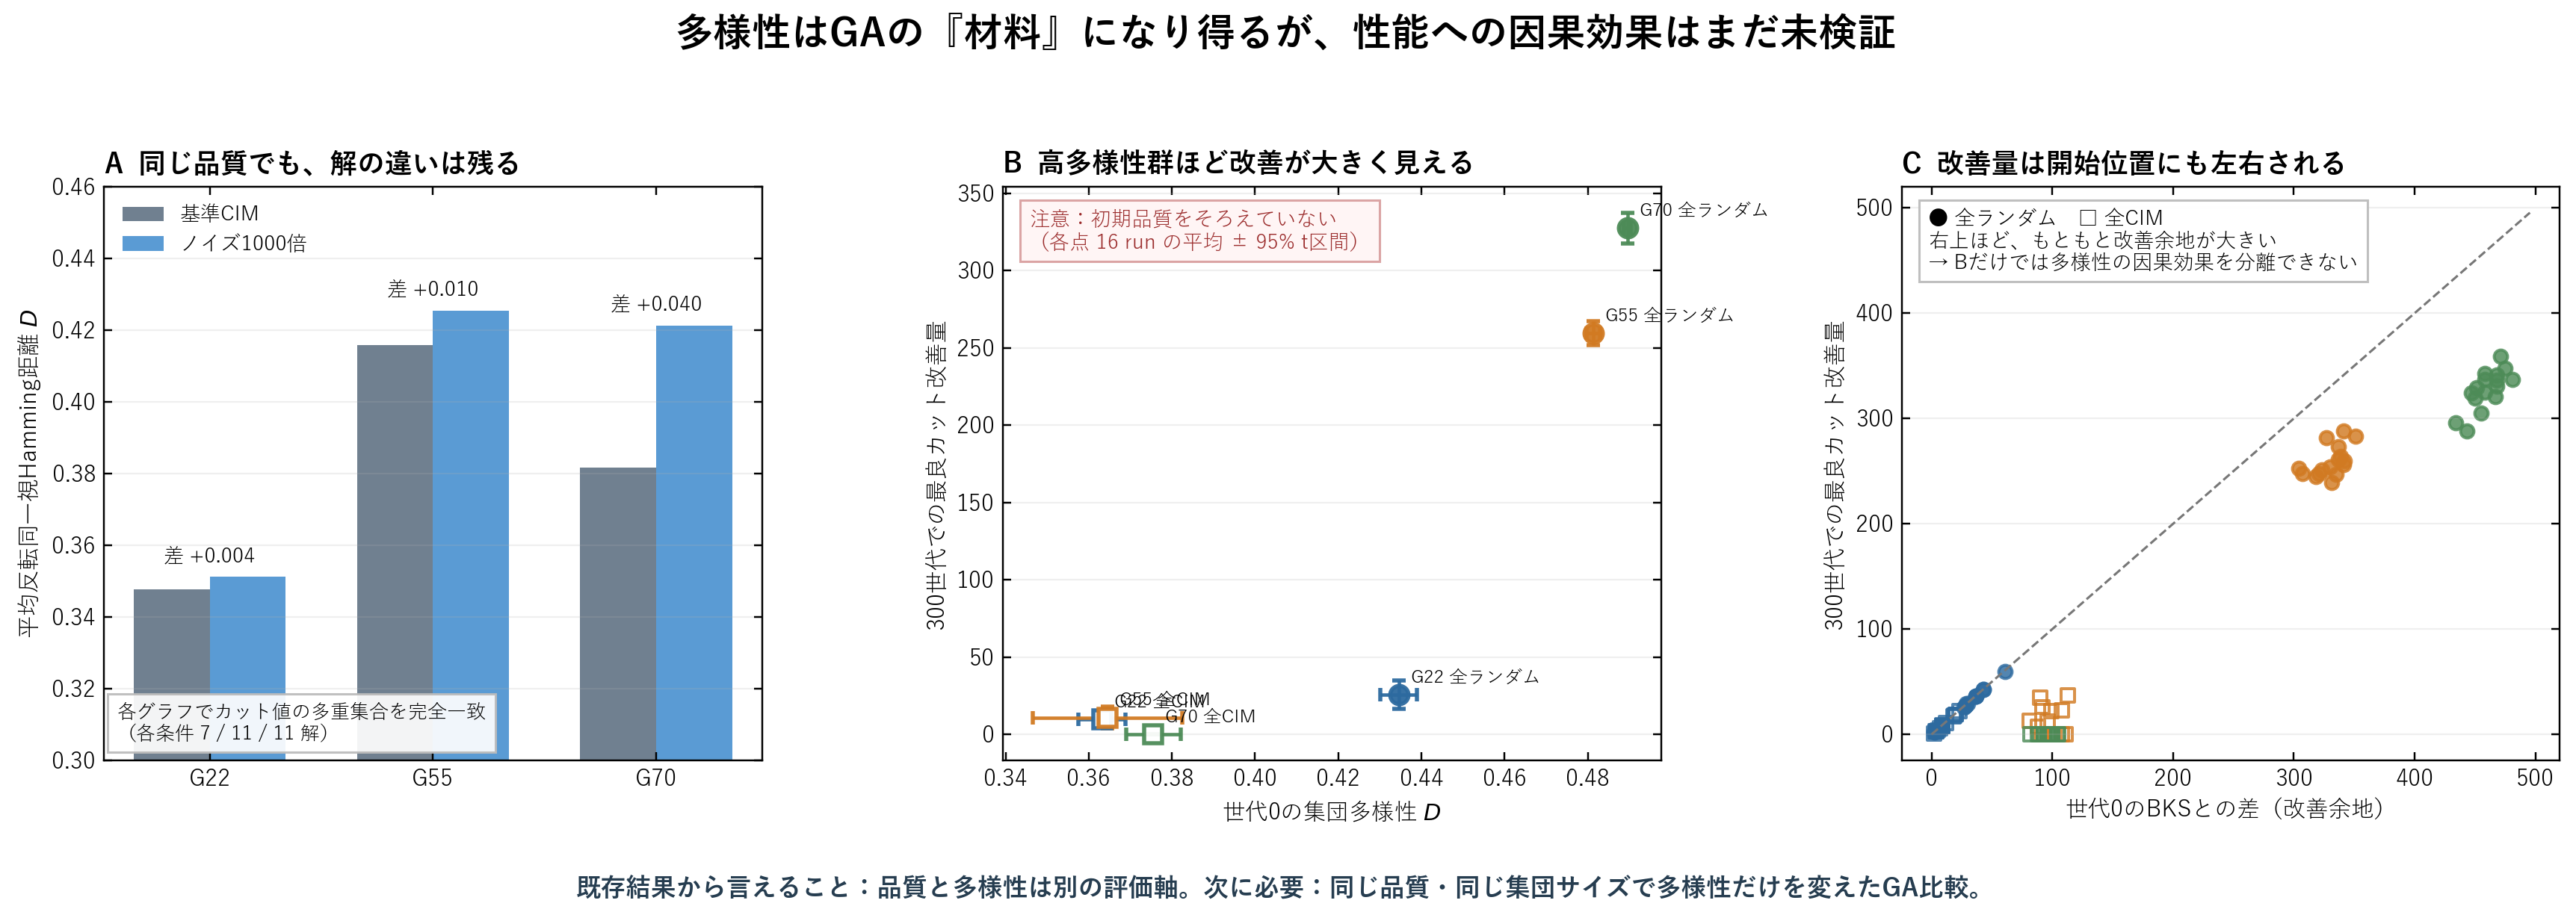
\includegraphics[width=0.985\linewidth,height=118mm,keepaspectratio]{evidence_map.png}
\end{center}

\textbf{読み方。} Aは「品質が同じでも異なる分割を持てる」ことを直接示す。Bでは高多様性群ほどGA改善が大きく見えるが、Cが示すように全ランダム群は開始時のカット値が低く、改善余地も大きい。したがって、Bの差を多様性の効果とは解釈できない。

\colorbox{yellow!18}{\parbox{0.97\linewidth}{\textbf{結論：}既存結果は、品質だけでなく多様性を測る研究動機を支持する。一方、「同じ品質なら多様な集団ほどGAの最終性能が高い」という因果命題は、まだ検証していない。}}

{\footnotesize 距離 $D$ は全反転を同一分割とする平均ペアHamming距離 $\min(H,N-H)/N$。誤差棒はrunを単位とする平均の95\% $t$区間。BKSは保存済み既知最良値。}

\clearpage
\heading{数値と研究上の位置づけ}{図に使った値。新しいGA実行や結果の補間は行っていない}

\textbf{1. カット値分布を完全一致させたCIM解集合}
\begin{center}\small
\begin{tabular}{lrrrrr}\toprule
問題 & 各条件の解数 & 同じ平均カット値 & 基準CIMの$D$ & ノイズ1000倍の$D$ & 距離差 \\\midrule
G22 & 7 & 13317.857 & 0.3476 & 0.3512 & +0.0036 \\
G55 & 11 & 10176.909 & 0.4158 & 0.4254 & +0.0095 \\
G70 & 11 & 9477.273 & 0.3817 & 0.4213 & +0.0396 \\
\bottomrule\end{tabular}
\end{center}

カット値ごとに両条件の少ない方の個数だけ保存順で抽出したため、平均だけでなくカット値の多重集合が一致する。距離による選別はしていない。ただし各条件7--11解の事後抽出であり、独立したGA反復ではない。

\textbf{2. GA軌跡の群平均（初期品質は未調整）}
\begin{center}\small
\begin{tabular}{llrrrr}\toprule
問題 & 初期集団 & 世代0の$D$ & 世代0のBKS差 & 300世代の改善量 & 最終BKS差 \\\midrule
G22 & 全ランダム & 0.4345 & 26.44 & 25.75 & 0.69 \\
G22 & 全CIM & 0.3632 & 10.81 & 9.94 & 0.88 \\
G55 & 全ランダム & 0.4813 & 330.25 & 259.50 & 70.75 \\
G55 & 全CIM & 0.3645 & 97.94 & 10.94 & 87.00 \\
G70 & 全ランダム & 0.4895 & 459.50 & 327.44 & 132.06 \\
G70 & 全CIM & 0.3755 & 95.81 & 0.00 & 95.81 \\
\bottomrule\end{tabular}
\end{center}

全ランダムと全CIMは同一GA設定、各16 run、300世代だが、世代0の品質をそろえていない。特にG55・G70では全ランダム群の改善余地が大きい。G70の全CIM群は16 runすべてで改善量0だったが、これは「多様性があれば改善する」とも「多様性が無意味」とも単独では言えない。

\textbf{3. 次に必要な検証}

同じカット値の多重集合、同じ集団サイズ、同じGA設定・計算予算を固定し、平均距離だけが低い／高い初期集団を複数構成する。対応する乱数で、(i) 最終カット、(ii) 最良値への到達世代、(iii) 交叉直後の新規性、(iv) 局所探索後の改善量を比較する。この比較で初めて、「改善につながる違い」を多様性指標が捉えるかを検証できる。

\textbf{出典と再現性}

同品質データ：\path{results/2026-09-14/cim_diversity_evidence/v2_G22_G55_G70_matched_r1000_discussion}。GA軌跡：\path{results/2026-09-14/ga_diversity_trajectory/v1_G22_G55_G70_nt16_gen300_measured}。元実験では864集団の距離と8352個体のカット値を独立照合済み。再解析コードと入力SHA-256は本PDFと同じフォルダに保存した。
\end{document}
